%%%%%%%%%%%%%%%%%%%%%%%%%%%%%%%%%%%%%%%%%%%%%%%%%%%%%%%%%%%%%%%%%%%%%%
% How to use writeLaTeX: 
%
% You edit the source code here on the left, and the preview on the
% right shows you the result within a few seconds.
%
% Bookmark this page and share the URL with your co-authors. They can
% edit at the same time!
%
% You can upload figures, bibliographies, custom classes and
% styles using the files menu.
%
% If you're new to LaTeX, the wikibook is a great place to start:
% http://en.wikibooks.org/wiki/LaTeX
%
%%%%%%%%%%%%%%%%%%%%%%%%%%%%%%%%%%%%%%%%%%%%%%%%%%%%%%%%%%%%%%%%%%%%%%

\RequirePackage[no-math]{fontspec}

\documentclass{tufte-handout}

%\geometry{showframe}% for debugging purposes -- displays the margins
\usepackage{amsmath}

% Set up the images/graphics package
\usepackage{graphicx}
\setkeys{Gin}{width=\linewidth,totalheight=\textheight,keepaspectratio}


\usepackage{color, colortbl}

%Portuguese-specific commands
%--------------------------------------
\usepackage[english, portuguese]{babel}
\selectlanguage{portuguese}
%--------------------------------------
 
%Hyphenation rules
%--------------------------------------
\usepackage{hyphenat}
\hyphenation{mate-mática recu-perar}
%--------------------------------------


% fix pro tufte no xetex (q preciso para fontes customizadas)
% https://tex.stackexchange.com/a/202189
\usepackage{ifxetex}
\ifxetex
  \newcommand{\textls}[2][5]{%
    \begingroup\addfontfeatures{LetterSpace=#1}#2\endgroup
  }
  \renewcommand{\allcapsspacing}[1]{\textls[15]{#1}}
  \renewcommand{\smallcapsspacing}[1]{\textls[10]{#1}}
  \renewcommand{\allcaps}[1]{\textls[15]{\MakeTextUppercase{#1}}}
  \renewcommand{\smallcaps}[1]{\smallcapsspacing{\scshape\MakeTextLowercase{#1}}}
  \renewcommand{\textsc}[1]{\smallcapsspacing{\textsmallcaps{#1}}}
\fi

% \usepackage{eulervm}
\usepackage{mathspec}
\setmainfont[
    Path=./Literata/,
    BoldFont=Literata-Bold,
    ItalicFont=Literata-Italic,
    BoldItalicFont=Literata-BoldItalic,
]{Literata-Regular}
\setmathfont(Digits,Latin)[Path=./Literata/,Scale=MatchLowercase]{Literata-Italic}

\title{Letras que ecoam a fala: tipografia modulada por prosódia}
%\title{A voz na letra: tipografia modulada pela fala}

\author{Caluã de Lacerda Pataca, Paula Dornhofer Paro Costa}
\date{24 de novembro de 2019}  % if the \date{} command is left out, the current date will be used

% The following package makes prettier tables.  We're all about the bling!
\usepackage{booktabs}

% The units package provides nice, non-stacked fractions and better spacing
% for units.
\usepackage{units}

% The fancyvrb package lets us customize the formatting of verbatim
% environments.  We use a slightly smaller font.
\usepackage{fancyvrb}
\fvset{fontsize=\normalsize}

% Small sections of multiple columns
\usepackage{multicol}

% Provides paragraphs of dummy text
\usepackage{lipsum}

% These commands are used to pretty-print LaTeX commands
\newcommand{\doccmd}[1]{\texttt{\textbackslash#1}}% command name -- adds backslash automatically
\newcommand{\docopt}[1]{\ensuremath{\langle}\textrm{\textit{#1}}\ensuremath{\rangle}}% optional command argument
\newcommand{\docarg}[1]{\textrm{\textit{#1}}}% (required) command argument
\newenvironment{docspec}{\begin{quote}\noindent}{\end{quote}}% command specification environment
\newcommand{\docenv}[1]{\textsf{#1}}% environment name
\newcommand{\docpkg}[1]{\texttt{#1}}% package name
\newcommand{\doccls}[1]{\texttt{#1}}% document class name
\newcommand{\docclsopt}[1]{\texttt{#1}}% document class option name



\makeatletter
\renewcommand{\fnum@figure}{Fig.~\thefigure}
\renewcommand{\fnum@table}{Tabela~\thetable}
\makeatother

\newcommand{\num}[1]{\textsc{(\oldstylenums{#1})}}



\begin{document}

\maketitle% this prints the handout title, author, and date

\begin{abstract}
\noindent Mollis a vitae sem vestibulum dictumst gravida a a scelerisque ad molestie primis ullamcorper a a. Mi adipiscing in eu a molestie cras blandit dui a dui natoque mollis parturient ultricies vel. Per tellus dis posuere faucibus a etiam velit ullamcorper rhoncus commodo in potenti sed in. A parturient neque neque a suscipit vestibulum facilisi lobortis dis viverra sem pretium phasellus dis parturient vestibulum dui at nibh imperdiet consectetur mauris ad magna condimentum in. Senectus at ut convallis varius enim morbi a nascetur vivamus himenaeos tristique a velit feugiat dapibus cubilia a ornare euismod eu augue id a a primis at. Sociis vestibulum erat duis quam mus vestibulum dui scelerisque tortor nulla natoque suspendisse erat adipiscing a tellus a duis erat eu pulvinar vestibulum consectetur nibh molestie curabitur congue. A ut varius egestas a proin condimentum adipiscing integer consectetur a amet consectetur ad mi sed hac nam quis adipiscing eleifend imperdiet lobortis lacinia varius penatibus a. Interdum et nam condimentum dapibus sed hac mi accumsan dolor vel sagittis convallis nisi id nostra nisl accumsan condimentum condimentum et mi adipiscing. Mauris ipsum arcu justo bibendum parturient a parturient ultricies pulvinar a suspendisse a a nisi a. Parturient volutpat duis cras netus parturient ut ad dui eros aliquet dolor ad cubilia justo a laoreet a posuere a diam lacinia porta.
\end{abstract}

%\printclassoptions

\section{Objetivos e justificativas do projeto de pesquisa}\label{sec:objetivos}
%\subsection{Headings}\label{sec:headings}

Em um filme, as legendas traduzem em texto aquilo que falam as personagens. Sons codificados tipograficamente dão acesso ao \textit{que} é dito, mas essa representação ignora \textit{como} as palavras são ditas. Nosso trabalho parte da ideia de que, dado que os sentidos do \textit{que se diz} são modificados pelo \textit{como se diz}, um sistema de legendas poderia buscar representações visuais que permitissem a seus espectadores intuir qualidades expressivas na voz das personagens e, assim, ter uma experiência audiovisual mais rica.

Tal sistema poderia ganhar usos como um componente de aplicações de acessibilidade, em especial considerando um público com deficiências auditivas que, a princípio, é excluído de toda uma dimensão expressiva quando assiste a conteúdos audiovisuais. Além desse uso mais restrito, imaginamos que, da mesma forma que as \textit{closed captions} trazem benefícios para públicos em geral, ouvintes ou não \citep{fiske_video_2015}, uma legenda expressiva poderia ganhar usos além das tecnologias assistivas.

Dentro deste projeto de mestrado, o escopo do trabalho circula em torno da criação de um protótipo que permita interpretar computacionalmente falas expressivas para então codificá-las, também computacionalmente, enquanto representações tipográficas. Além de desenvolvê-lo, buscaremos avaliar diferentes aspectos desse modelo ``prosódico-tipográfico'', visando tanto medir seus efeitos quanto melhor entendê-los.

\section{Revisão bibliográfica resumida}\label{sec:revisao_bibliografica}

Nosso estudo é fundado na noção de que a prosódia da fala compreende uma dimensão emocional. Trata-se de uma constatação simples: o mesmo trato vocal que molda a fala é parte de um corpo que, sob efeito de diferentes estados emocionais, se tensiona e relaxa de diversas maneiras. A emoção não é, claro, a única dimensão que modula os parâmetros acústicos da prosódia:\sidenote[][-3\baselineskip]{Ainda que não tenhamos tratado a questão nos dois primeiros experimentos já realizados, lidar com o fato de que variações prosódicas em geral compreendem diversos aspectos além da emoção é um desafio importante em nosso trabalho.} diferentes autores enquadram sob formas diversas as funções da prosódia \citep{schotz2002linguistic}, mas para nossos propósitos cabe citar três aspectos: linguístico, paralinguístico e extralinguístico: 

\begin{quotation}
    Enquanto o conteúdo verbal -- efetivamente o significado das palavras -- é considerado como informação linguística, o canal extralinguístico contém informações sobre o estado base do falante, e.g. uma pessoa grande (...) terá uma voz mais grave do que a de uma criança. Alguns parâmetros extralinguísticos são também determinados pela cultura do falante. (...) O canal paralinguístico carrega informações sobre desvios passageiros da linha de base típica (extralinguística), tais como (...) a expressão de emoções. \sidenote[][-8\baselineskip]{\begin{otherlanguage}{english}
    \textit{Whereas the verbal content, the actual meaning of the words, is thought of as linguistic information, the extralinguistic channel contains information about the speaker's basic state, e.g. a big person (...) will usually have a lower voice than a child. Some extralinguistic parameters are also determined by the culture of the speaker. (...) The paralinguistic channel carries information about momentary deviations from the usual (extralinguistic) baseline, such as (...) the expression of emotions.} \end{otherlanguage} \citep{quast2001automatic}}
\end{quotation}

A presença de aspectos emocionais na prosódia é explorada em \citet{SILVA2016}, onde um conjunto de áudios em português natural foi avaliado por brasileiros e suecos. Ainda que entre os brasileiros tenha havido maior grau de concordância nas respostas, os suecos, para quem o componente linguístico dos áudios era indiferente, também conseguiram decodificar emoções.

Essas três dimensões prosódicas (linguística, para- e extra-) são articuladas pela produção e recepção de três parâmetros acústico-perceptuais \sidenote[][-1\baselineskip]{Como mostra \citet{livroDoPlinio}, a relação entre produção e percepção não é linear e esses parâmetros se entrelaçam: mudanças em um causam diferenças de percepção em outro.}, que modificam cada sílaba em relação às demais: intensidade (mais fraca ou forte), \textit{pitch} (mais aguda ou grave) e duração (mais lenta ou rápida).

Parte dessas variações é codificada na linguagem escrita, parte não. Com efeito, a história da escrita acompanha inúmeras mutações em convenções -- inicialmente caligráficas, eventualmente tipográficas -- que, muitas vezes, estão relacionadas à variações na representação de atributos prosódicos. 

\begin{marginfigure}
  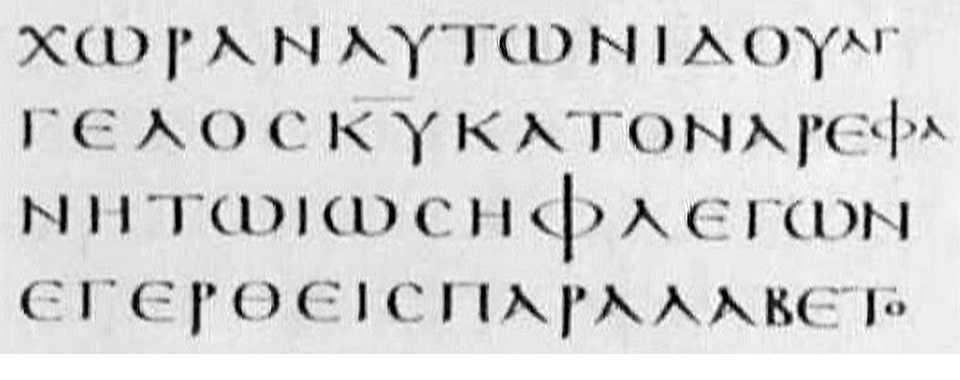
\includegraphics{imgs/codex.png}
  \caption{Trecho do \textit{Codex Vaticanus}, datado do século \textsc{iv}, exemplo de \textit{scriptio continua}. \citep{codex_vaticanus}}
  \label{cdx_vat}
\end{marginfigure}

Até que fossem introduzidos no século \textsc{vii}, não se usavam espaços ou outros sinais para separar as palavras, o texto um bloco fechado de letras -- a partir do que alguns historiadores avançam a teoria\sidenote{Popular, mas bastante controversa. Ver \citet{McCutcheon2015}.} de que a literatura na antiguidade era predominantemente acústica \citep{kuster2016}: a leitura se fazia necessariamente em voz alta pois só ao converter em sons o ``bloco'' este se tornaria compreensível. O texto então seria ``melhor percebido pelos ouvidos do que pelos olhos.'' \citep{nunlist1991}

Inovação medieval (ou não), a leitura silenciosa não é, como talvez se possa imaginar, desprovida de prosódia. Dentre as estruturas cerebrais envolvidas no processo de leitura, é surpreendente notar que, além das estruturas encarregadas do processamento semântico e ortográfico, a leitura demanda também aquelas tipicamente relacionadas à produção e processamento de sons \citep[cap.~7]{seidenberg2017}. Isso ocorre porque, mesmo quando lê silenciosamente, cabe ao leitor deduzir em sua voz interna uma representação sonora do texto, habilidade fundamentalmente relacionada à compreensão e interpretação do mesmo.

O bom funcionamento dessa ``voz'' interna é importante. Certos tipos de dislexia, por exemplo, parecem antes causados por problemas nessas estruturas fonológicas do que deficiências nas processamento de imagens, mesmo que se manifestem sob a forma de dificuldades na  leitura \citep[cap.~8]{seidenberg2017}. Ao contrário da noção vendida por certos cursos de leitura dinâmica de que uma leitura sem subvocalização traria ganhos de velocidade sem perdas na compreensão, o leitor experiente depende dessa voz interna para reduzir ambiguidades e facilitar a compreensão \citep[cap.~4]{seidenberg2017}. Finalmente, crianças em processo de alfabetização que leem de maneira monótona tendem a desenvolver problemas de compreensão \citep{bessemans2017}.

A partir da hipótese de que a falta de representação prosódica na tipografia seria um empecilho na alfabetização, a pesquisadora belga Ann Bessemans e seu grupo têm estudado um tipo de intervenção no texto que busca ajudar crianças a ler expressivamente. No estudo, codifica-se visualmente a prosódia na tipografia: texto em \textit{negrito} quando lido com maior volume, \textit{espremido} quando mais rápido, \textit{esticado} quando mais lento e \textit{elevado} quando agudo. Seus resultados iniciais mostram que as crianças conseguiram entender e integrar essas dicas visuais na sua leitura, indicando o potencial da abordagem como uma representação intuitiva da expressividade da voz. \citep{bessemans2017}

\citet{wolfel2015} criaram o \textit{Design de Tipos Orientado pela Voz} (\textsc{vdtd}, sigla para \textit{Voice Driven Type Design}), uma abordagem semelhante à de Bessemans mas de base computacional. Nela, mapearam atributos acústicos de cada fonema -- como intensidade, \textit{pitch} e velocidade -- em grafemas de uma fonte geométrica matematicamente modelada e cujos atributos podem ser manipulados. Em uma avaliação com leitores, foram encontrados indícios tanto de que as características da fala conseguiram ser impressas no texto quanto que uma abordagem nessa linha poderia ser usada para representar emoções presentes na voz. \sidenote[][-3\baselineskip]{O \textsc{vdtd} serviu como grande inspiração para nosso próprio trabalho, mas buscamos divergir no que consideramos duas falhas em sua abordagem: \num{1} o uso de uma tecnologia tipográfica própria é um grande empecilho para a eventual adoção da tecnologia nos já existentes ambientes de uso de tipografia digital; \num{2}~a avaliação foi construída principalmente com questionários onde um pequeno número de participantes fez autorrelatos de suas impressões, o que significa que os (pequenos) efeitos medidos são difíceis de generalizar.}

\citet{wolfel2015} discutem ainda algumas aplicações práticas de seu \textsc{vdtd}. Em volta de uma delas -- legendas moduladas pela voz, em especial quando apresentadas na mesma língua em que o vídeo é falado -- gravita nosso projeto. Esperamos aqui lançar contribuições para um cenário sobre o qual há benefícios amplamente documentos, como sintetiza \citet{fiske_video_2015}: filmes legendados produzem melhoras na compreensão, atenção e memória em diversos públicos: crianças, adultos ou idosos; leitores experientes ou em fase de aprendizado; falantes ou não da língua em questão; ouvintes ou com deficiências auditivas; etc.

Em especial, \citet{MurphyBerman1983} levantam um desafio relacionado às legendas que nos parece certeiro: em seu estudo, testaram se, para crianças surdas e alfabetizadas, a presença de \textit{closed captions} se traduzia em um entendimento mais aprofundado de um programa de televisão, especificamente em relação ao seu conteúdo \textit{afetivo}. Os resultados indicaram que sim. Ao final, as autoras se perguntaram sobre quais efeitos gráficos conseguiriam traduzir visualmente no texto a ``rica informação tonal que é negada às crianças surdas por não terem acesso à trilha sonora''. Nosso projeto, acreditamos, poderá apontar um~caminho.

\section{Metodologia utilizada}\label{sec:metodologia}

\subsection{Extração e representação de prosódia}\label{sec:met_extract_represent}

Nossa abordagem pede que se construa um algoritmo que abstraia numericamente certos elementos acústicos que sirvam de bons representantes da expressão vocal para, então, mapeá-los visualmente enquanto tipografia. Pelo que já foi discutido, a prosódia traz um bom conjunto de parâmetros acústicos (\textit{features}), mas considerando que nossa unidade mínima de mapeamento visual será a letra (ou, mais provavelmente, a sílaba), um ponto adicional a favor de se usar \textit{features} prosódicas é que elas podem ser tomadas em nível local (da sílaba) em oposição às de nível global (da frase), como discutem \citet{rao2010characterization}.

Na versão atual do software, usamos as seguintes \textit{features}:
\begin{enumerate}
    \item Amplitude, calculada em decibéis como a média do \textit{Root Mean Square} (\textsc{rms}) de cada sílaba;
    \item \textit{Pitch}, calculada em Hz a partir da frequência fundamental ($f_0$) média, calculada usando o método \textsc{swipe} da biblioteca \textit{pysptk}, aplicado em janelas de 512 amostras com limite de frequências entre 75 e 600 Hz.
    \item Duração, em milisegundos.
\end{enumerate}

\begin{marginfigure}[-7\baselineskip]
  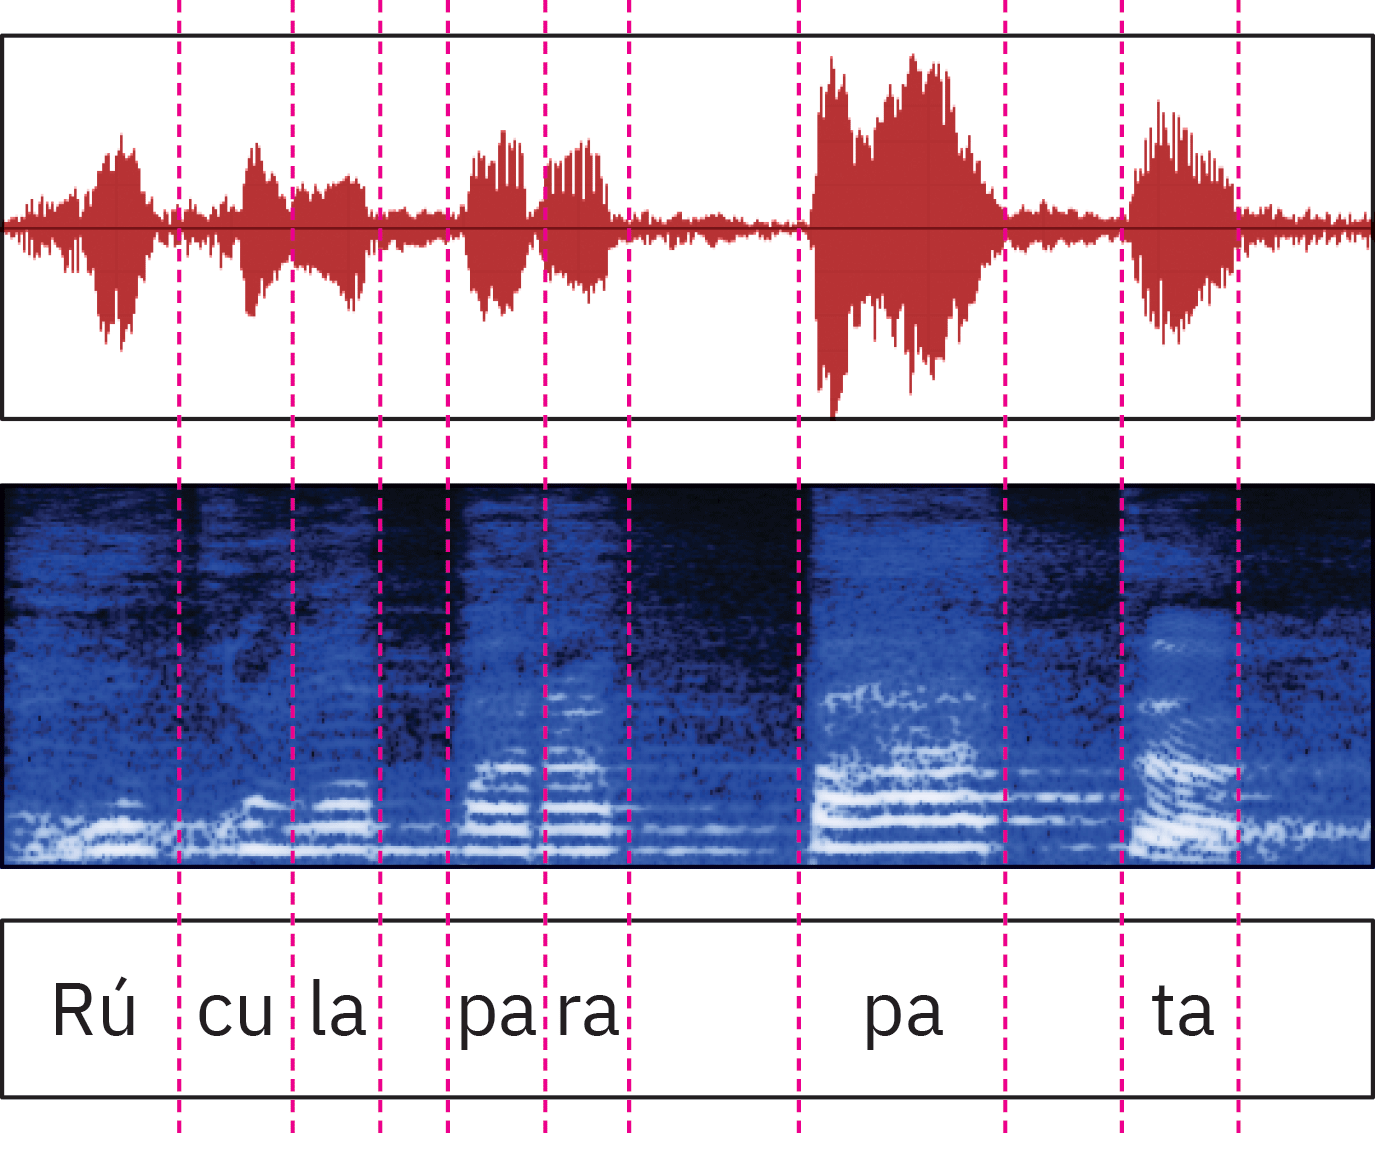
\includegraphics{imgs/diag-extracao.png}
  \caption{Visualização esquemática de um arquivo de áudio com a frase ``Rúcula para pata'', ressaltando três de seus aspectos acústicos, de cima para baixo: amplitude, frequências e duração silábica.}
  \label{diag_extracao}
\end{marginfigure}

Em versões posteriores do software, as seguintes melhorias devem ser consideradas:

\begin{enumerate}
    \item Se atualmente as \textit{features} estão organizadas em torno da fala, futuramente faria sentido reorientá-las em direção à audição. \citet{livroDoPlinio} discute certas diferenças desses dois polos e seria importante explorar compensações que levem em conta efeitos psicoacústicos conhecidos -- e.g. a resposta de frequências do ouvido humano é não-linear, o que pode ser melhor modelado usando-se semitons ao invés de Hz; variações de $f_0$ causam a percepção de maior duração; a sensação de \textit{pitches} agudos é amplificada por maiores volumes; etc.
    
    \item \textsc{rms} é uma medida pouco resistente a diferenças de gravação não relacionadas à diferenças de esforço vocal. Um falante que tenha a voz em volume constante mas que se aproxime ou se distancie do microfone terá um \textsc{rms} artificialmente modificado. As medidas de intensidade \textit{relativas} -- calculadas pela diferença de intensidade entre faixas de baixa e alta frequência -- são mais robustas ao ambiente de gravação.
\end{enumerate}

A segunda parte do software envolve o mapeamento visual dessas \textit{features} no texto. Como \citet{wolfel2015}, consideramos que o mapeamento das variáveis contínuas do áudio nas poucas\sidenote[][-2\baselineskip]{Há de fato algumas raras famílias tipográficas que possuem tantos pesos a ponto de se poder questionar se a diferença entre cada um é grande o suficiente para ser percebida por si só (e.g. a Lucida Sans, que em sua versão completa tem 18 pesos entre o \textit{UltraThin} e o \textit{UltraBlack}). Mesmo que fosse esse o caso, nossa abordagem ainda se justificaria por, primeiro, manter-se agnóstica em relação a esta ou aquela fonte e, segundo, porque, propondo combinações de variações em eixos que não só o \textit{peso}, acabamos indo além do que se oferece nas mais extensas famílias tipográficas disponíveis.} categorias tipicamente disponíveis em uma fonte digital comum (e.g. peso leve, normal e negrito) levaria a resultados com poucas nuances, sem ecoar visualmente as sutilezas presentes na fala e que supomos importantes para a apreensão afetiva por parte do ouvinte.

Com isso, podemos considerar dois requisitos a partir dos quais deverá emergir a solução técnica para essas representações: \num{1} para as modulações tipográficas, não se deve discretizar (ao menos não perceptualmente) as \textit{features} que vierem do áudio, ou seja, a tipografia deverá conseguir ecoar mesmo mudanças sutis na fala; \num{2} deve ser possível que cada tipo de modulação funcione de maneira independente uma da outra na representação, pois também independentes entre si poderão ser as \textit{features} vindas do~áudio. \sidenote{É igualmente plausível que uma palavra seja dita de maneira forte e rápida \textit{ou} de maneira forte a lenta, por exemplo, e a tipografia deverá conseguir ecoar as duas características de maneira independente uma da outra.}

Dada essa demarcação, excluímos, pela complexidade envolvida, o desenvolvimento de um algoritmo que reconstruísse o desenho da letra a partir de modificações em sua estrutura interna, como o fazem \citet{wolfel2015}; pelos motivos citados por \citet{haralambous1993}, trabalhar com a \textsc{metafont}, de Donald Knuth, também seria infrutífero.

Optamos, então, por aplicar as modulações em \textit{variable fonts}. Há já implementações em diferentes ambientes -- as definições de \textsc{css} que definem como usar \textit{variable fonts} já funcionam nos principais navegadores\sidenote[][-4\baselineskip]{~88\% dos usuários já teriam acesso à tecnologia na internet. Ver: https://caniuse.com/\#feat=variable-fonts, acesso em 27/11/19.}, assim como  bibliotecas código livre para C e Python.

Publicada em setembro de 2016, a versão 1.8 da especificação OpenType define as \textit{variable fonts}. Nelas, o tipógrafo cria ``eixos'' -- dimensões que guiam diferentes tipos de modulação visual que poderá sofrer cada caractere. Uma fonte pode ter uma quantidade arbitrária de eixos, que operam de maneira independente uns dos outros \citep{varfontssepcs}. 

\begin{marginfigure}
  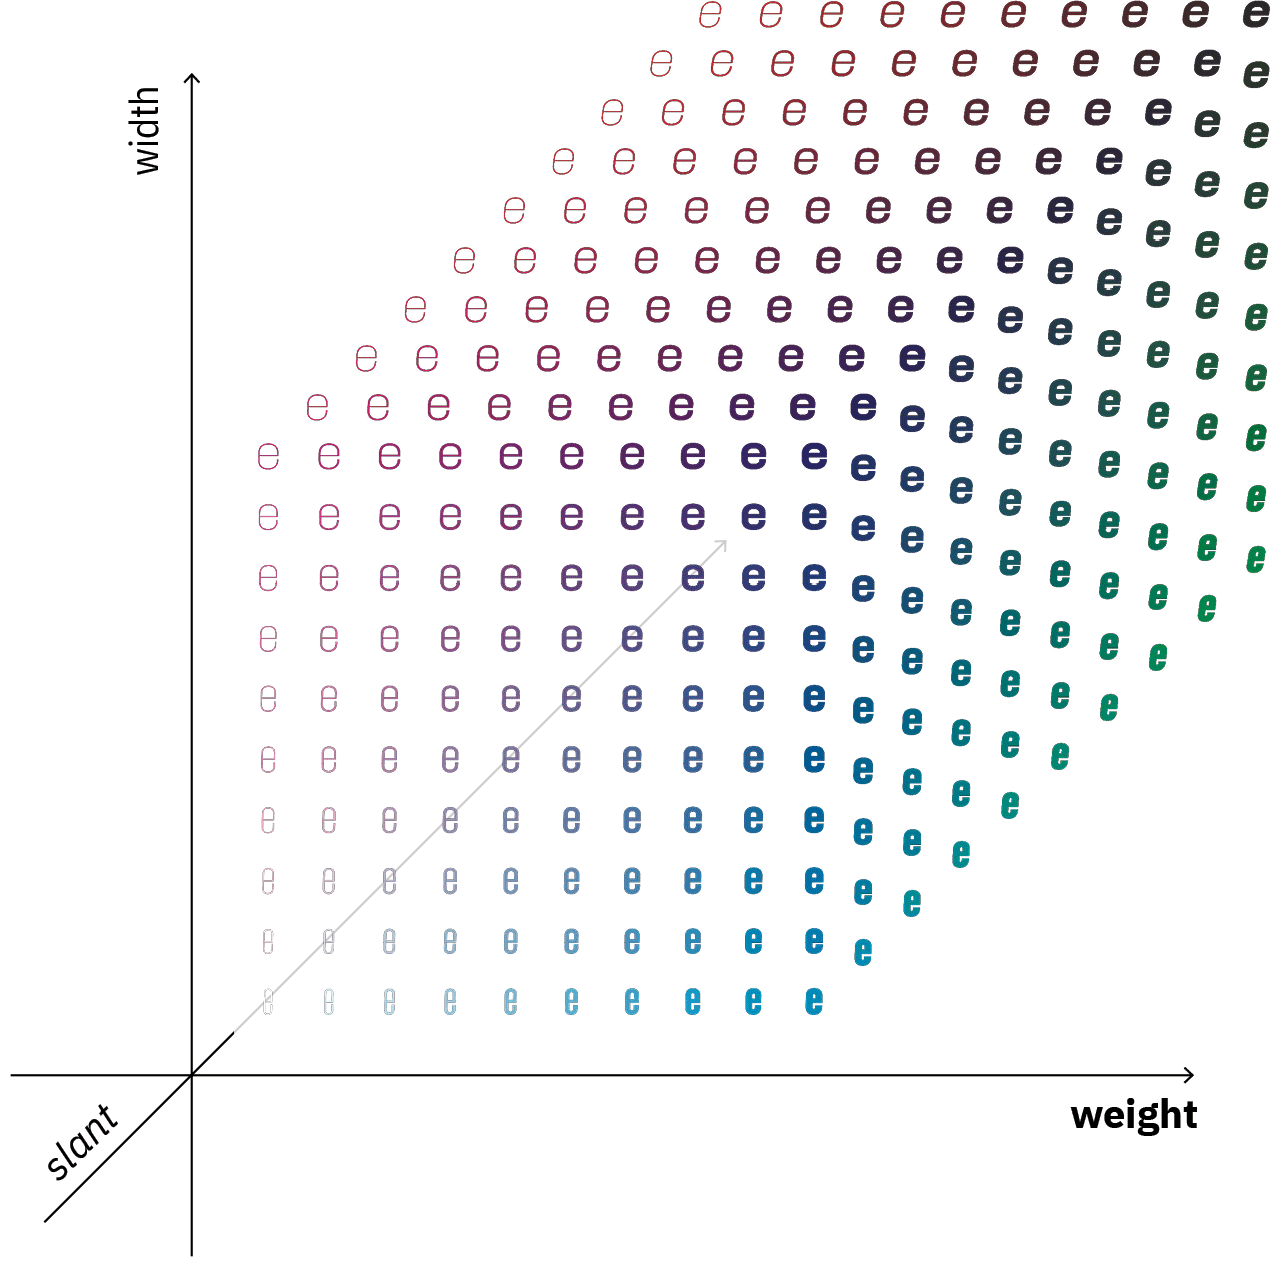
\includegraphics{imgs/grafico-var.png}
  \caption{Como o glifo `e' se modifica conforme variam os valores de seus três eixos?}
  \label{grafico_var}
\end{marginfigure}
    
Internamente, em uma \textit{variable font} estão definidos os pontos que compõe o desenho de cada letra em sua posição central, \textit{neutra}, além das instruções sobre como cada um desses pontos deve se transformar quando um dado eixo tiver definido seu menor e maior valores possíveis, com as posições intermediárias sendo interpoladas.
    
Por exemplo, uma fonte contendo os eixos \textit{peso} e \textit{largura horizontal} poderá oferecer uma versão estreita e grossa (largura no mínimo, peso no máximo), ou outra estendida e fina (largura no máximo, peso no mínimo), além das posições intermediárias.

\begin{marginfigure}[\baselineskip]
  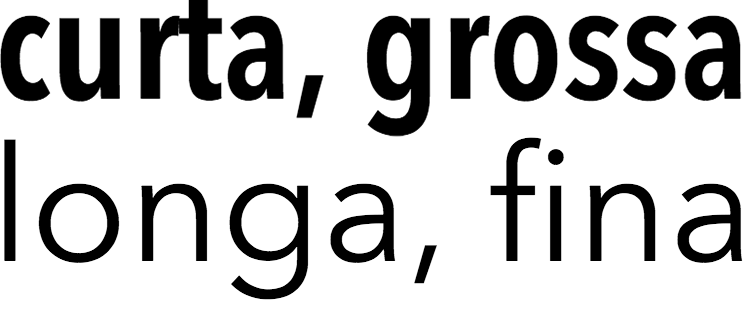
\includegraphics{imgs/curta-grossa-longa-fina.png}
  \caption{Variação em dois eixos (\textsc{wght}, ou peso, e \textsc{wdth}, ou largura), na fonte \textit{Avenir Next VF}.}
  \label{curta_grossa_longa_fina}
\end{marginfigure}

\subsection{Experimento \#1: Card sorting e entrevistas com designers}\label{sec:met_exp_1}

O propósito da primeira avaliação seria investigar que influências nosso modelo prosódico-tipográfico teria na interpretação de um texto. Para isolar os efeitos da forma tipográfica, buscamos frases cujo conteúdo textual fosse pouco expressivo, ou seja, onde o efeito \textit{linguístico} fosse mínimo. Inversamente, as frases deveriam ter a voz carregada de emoção, ou seja, com uma dramaticidade vocal que produzisse grandes variações visuais no desenho tipográfico. Optamos por usar bases de frases/áudio previamente criadas (os meandros da criação de uma nova fogem ao que queremos explorar).

Assim, ainda que criada sob motivações estranhas às nossas, escolhemos a base criata por \citet{pdpcosta2015}. Nela, e cumprindo o primeiro requisito, havia 10 frases sem relação entre si e ``neutras, de modo que cada uma permita [pelos atores] a interpretação de diferentes emoções'' \citet[p.50]{pdpcosta2015}. Cumprindo nosso segundo requisito, as frases foram lidas por quatro atores, cada um buscando representar as 6 emoções -- tristeza, medo, surpresa, repulsa, raiva e alegria -- da tipologia ``Big Six'' \citep{ekman1970universal}.~\sidenote{Entre outras, a base inclui também leituras neutras, que usamos no segundo experimento.} Para nosso experimento, escolhemos quatro frases e, para minimizar variações entre leitores, fixamos os áudios nos de uma das atrizes.

Aplicamos o seguinte mapeamento de parâmetros prosódicos para eixos tipográficos:

\begin{itemize}
    \item Amplitude \enskip \textrightarrow \enskip \textit{Weight} (peso) -- como em \citet{wolfel2015} e \citet{bessemans2017};
    
    \item Duração \enskip \textrightarrow \enskip \textit{Width} (largura horizontal) -- que em \citet{van2006towards} é associada à ideia de velocidade;
    
    \item Frequência fundamental \enskip \textrightarrow \enskip \textit{Slant} (inclinação) -- este uso uma aposta nossa. Não encontramos exemplos de seu uso na representação de prosódia, mas quisemos evitar o uso que \citet{bessemans2017} faz do deslocamento de linha de base para representar \textit{pitch}, por questões que esse uso traria em textos mais longos (ainda que tenhamos voltado atrás no segundo experimento);
\end{itemize}

\begin{marginfigure}
  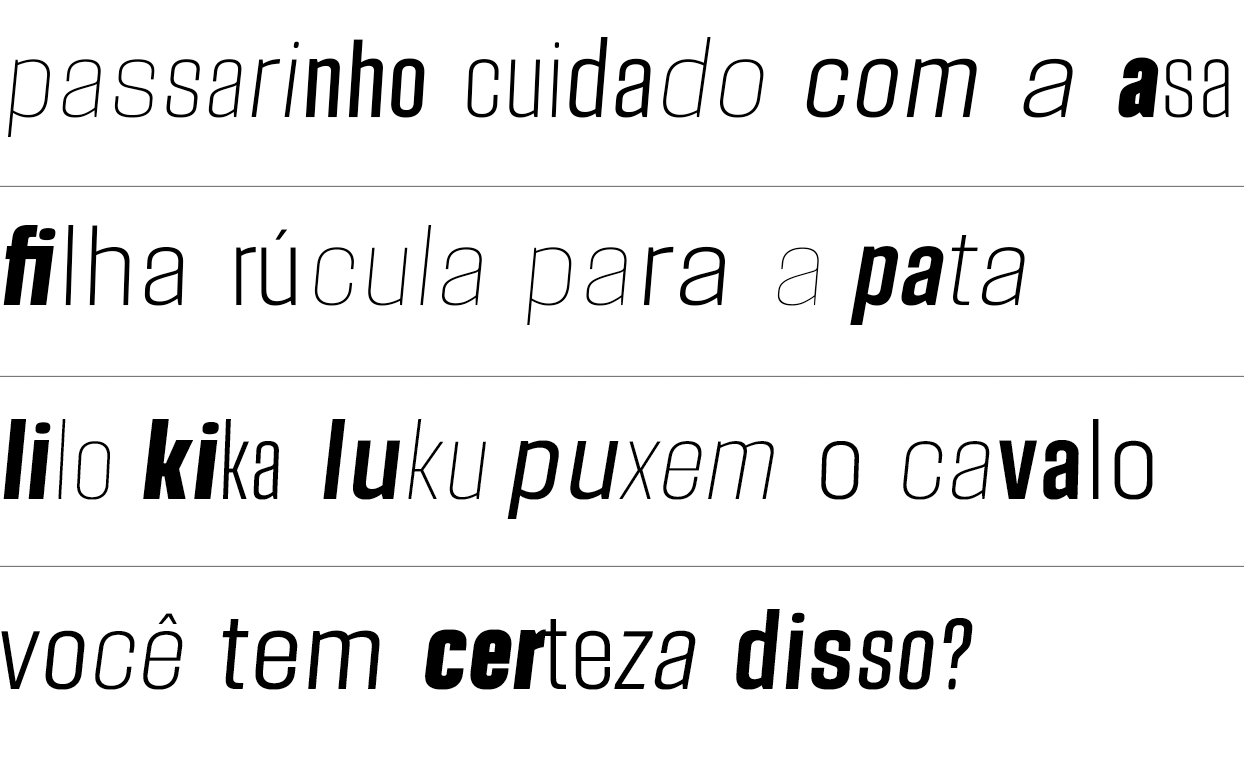
\includegraphics{imgs/exemplos-frases-2.png}
  \caption{Exemplo de cada frase usada nos cartões com aplicação do modelo prosódico-tipográfico.}
  \label{exemplo_frases}
\end{marginfigure}

Os seis arquivos de áudio para cada uma das quatro frases foram então processados e os textos resultantes, com a tipografia modificada pela fala da atriz, impressos em cartões de papel tamanho A5. Na Figura~\ref{exemplo_frases}, apresentamos um exemplar de cada uma das frases usadas. 

Para a avaliação realizaríamos sessões de \textit{card sorting}, uma técnica de exploração e avaliação de taxonomias comum no campo da \textsc{ihc} (Interação Humano-Computador) para arquitetar sites ou softwares, mas que tem aplicabilidade em outras áreas sempre que se queira investigar como diferentes pessoas formulam modelos mentais para estruturar algum conjunto de dados \citep{about_cardsorting}.

Em suas duas formas mais comuns, a \textit{open} e \textit{closed card sorting}, faz-se uma atividade na qual um grupo de pessoas\sidenote{\textit{Stakeholders} que podem ou não ser especialistas -- em algumas situações, busca-se um público leigo para desvendar como ele organiza mentalmente as informações de uma área na qual seu conhecimento é superficial.}, uma a uma, organiza um conjunto de cartões de papel em diferentes envelopes. Dentro da taxonomia que se quer investigar, cada cartão representa um dado e cada envelope representa uma categoria. Estas podem ser pré-definidas (\textit{closed cart sorting}) ou criadas no ato pelos próprios participantes (\textit{open card sorting}). Nos interessava a primeira opção: um dos usos típicos da \textit{closed card sorting} é testar se uma dada taxonomia é adequada para descrever um conjunto de informações. Em nosso caso, essa taxonomia seria as seis emoções a partir das quais os atores encenaram cada gravação de áudio. No experimento, esperávamos descobrir quão bem as ``Big Six'' serviriam para descrever os textos que foram modulados visualmente de acordo com o áudio.

Para analisar os resultados, decidimos pelo método de comparação de \textit{edit distances}. Esta é uma medida quantitativa na qual obtém-se a soma de operações de troca de posição necessárias para converter um arranjo de cartões em outro, ou seja, um índice da divergência entre os conjuntos -- útil para medirmos quão convergente cada participante foi em relação às ``Big Six.'' \citep{nawaz2012}

Se encontrássemos nos dados algum nível razoável de convergência entre as emoções implícitas em cada cartão e a forma como os participantes as interpretaram e organizaram, teríamos bons indícios de que a modulação visual da tipografia conseguiu imprimir um sentido afetivo coerente aos textos.

Também nos interessou usar o \textit{card sorting} pois, além do bom custo-benefício (é relativamente rápido e barato \citep{goodman2006card}), sendo um teste presencial, nos permitiria observar os participantes e realizar breves entrevistas semi-estruturadas ao final de cada sessão, complementando os dados numéricos.

Antes do início de cada sessão os participantes seriam informados de que haveria nos cartões uma correspondência entre a forma tipográfica e certas características da voz de uma atriz que lera previamente os textos -- não informamos maiores detalhes. Para cada emoção haveria um envelope rotulado e os participantes seriam instruídos a depositar cada cartão na ``emoção'' correspondente a seu desenho tipográfico. 

Como dito, ao final de cada sessão realizaríamos breves entrevistas semi-estruturadas, buscando levantar possíveis estratégias usadas pelos participantes na organização dos cartões, além de investiga possíveis modelos mentais formulados para explicar o funcionamento do mapeamento fala-tipografia.

\subsection{Experimento \#2: Associação entre emoções, \textit{features} prosódicas e eixos tipográficos}\label{sec:met_exp_2}

O segundo experimento foi planejado após percebermos, pela coleta e análise de dados do primeiro, que seria necessária uma investigação de foco mais estreito para entender melhor os componentes de nosso modelo prosódico-tipográfico. Como nos dados que tínhamos então não conseguimos isolar o impacto de cada eixo tipográfico como representação de cada \textit{feature} prosódica para cada emoção, no segundo experimento pretendemos isolá-los, explorando, um-a-um, como a interação desses parâmetros influenciava a percepção da tipografia. 

Pela quantidade de possibilidades a se testar, e considerando as dificuldades logísticas que notamos no \textit{card sort}, migramos para um ambiente online -- uma plataforma que criamos e que nos permitiria testar as inúmeras combinações possíveis entre emoção, prosódia e tipografia. 

Nossos objetivos eram então \num{1} descobrir se os participantes interpretariam de maneira consistente as relações entre emoções no áudio e modulações tipográficas, \num{2} explorar relações entre padrões nas \textit{features} e padrões nas preferências dos participantes e \num{3} ajudar a formular hipóteses sobre o sucesso (ou eventual fracasso) da capacidade de cada eixo tipográfico representar cada \textit{feature} prosódica.

Além dos três eixos tipográficos já testados no primeiro experimento, introduzimos um quarto, que chamamos de \textit{baseline shift}, ou deslocamento de linha de base. Nos inspiramos pela notação informal de melodia em canções brasileiras usada por \citet{tatit} que, supomos, seria especialmente adequada para representação de $f_0$. Na figura~\ref{mods-exp-2} vemos as quatro modulações tipográficas.

\begin{marginfigure}[-6\baselineskip]
  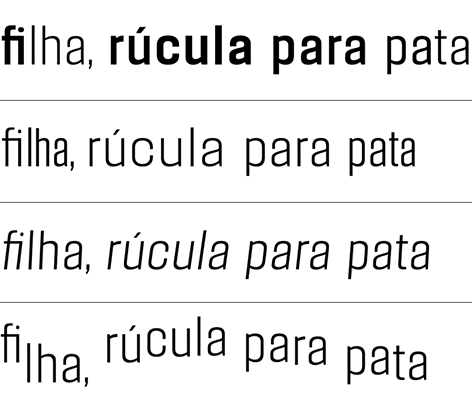
\includegraphics{imgs/modulacoes-experimento-2.png}
  \caption{As quatro modulações tipográficas testadas no segundo experimento. Respectivamente: \textit{weight}, \textit{width}, \textit{slant} e \textit{baseline shift}. NOte que elas não estão combinadas entre si, pois assim foram usadas no experimento.}
  \label{mods-exp-2}
\end{marginfigure}

\begin{marginfigure}[\baselineskip]
  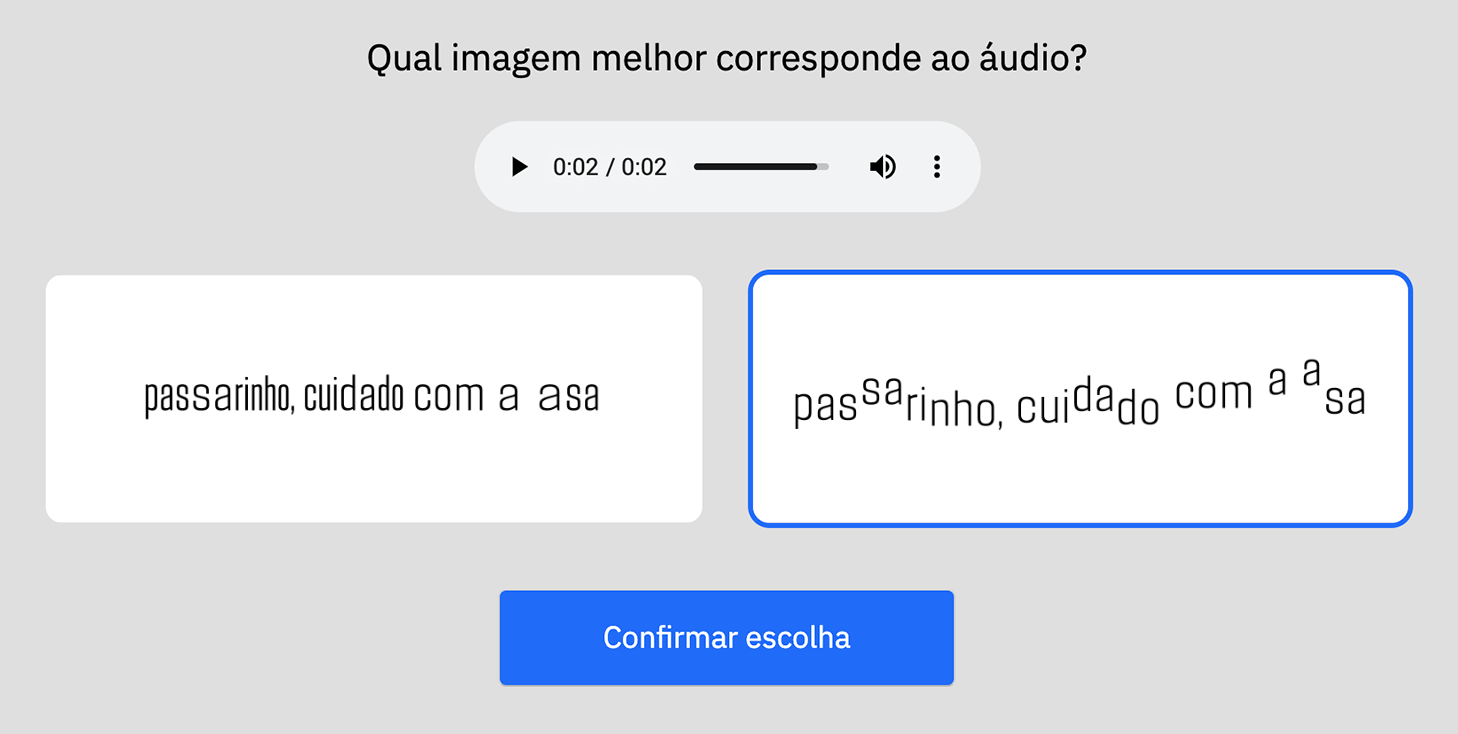
\includegraphics{imgs/test_screenshot2.png}
  \caption{No segundo experimento, participantes tinham de escolher (30 vezes) qual imagem melhor correspondia a um áudio.}
  \label{screenshot}
\end{marginfigure}


A Figura~\ref{screenshot} mostra uma captura de tela do teste. Nela, dois cartões contendo a tipografia modulada eram exibidos, ambos com a mesma frase e sobre a qual uma das quatro modulações (\textit{weight}, \textit{width}, \textit{slant} e \textit{baseline shift}) havia sido aplicada. Em cima das duas frases havia um tocador de áudio, sempre contendo o áudio da frase a partir da qual haviam sido extraídas as \textit{features} prosódicas. Detalhe importante: a cada rodada só se extraía \textbf{uma} \textit{feature}, aplicada em cada cartão a apenas \textbf{um} eixo tipográfico. A pergunta que se fazia era ``Qual imagem melhor corresponde ao áudio'' e, com as respostas, geraríamos um conjunto de dados nos dizendo que: 

\begin{quote}
    ...participante [A] escolheu o eixo [B] ao invés do eixo [C], ambos representando a \textit{feature} [D] extraída da frase [E] e na qual fora atuada a emoção [F].
\end{quote}

Para reduzir a gama de possibilidades (e, assim, exigir uma quantidade menor de participantes antes de se chegar a resultados estatisticamente significantes), consideramos apenas duas \textit{features} (amplitude e $f_0$), quatro emoções (raiva, alegria, tristeza e surpresa, além do áudio neutro, que introduzimos) e duas frases (\textit{Filha, rúcula para pata} e \textit{Passarinho, cuidado com a asa}). Em relação às \textit{features}, vimos que nos áudios escolhidos \textit{duração} tinha uma correlação negativa forte com \textit{amplitude} e, talvez, pudesse ser excluída no teste. Com as emoções, também: \textit{nojo} e \textit{medo} nos áudios escolhidos tinham padrões prosódicos semelhantes ao de outras das emoções e, portanto, foram descartados.

No teste em si havia então 5 emoções × 4 eixos tipográficos × 2~frases, equivalendo a 40 cartões, combináveis de 60 maneiras. Em um teste piloto chegamos a 30 rodadas por participante como um bom meio termo entre querer cobrir o máximo número possível de combinações e quão cansativo podia ser o experimento. Dividimos o teste em duas rodadas, cada qual testando uma das \textit{features}. Para compensar efeitos de cansaço ou mesmo inaptitude no início, a ordem e pares eram sempre sorteados.\sidenote[][-4\baselineskip]{Durante o teste fazíamos algumas medições relacionadas ao uso da plataforma. Duas delas -- tempo gasto por rodada e quantidade de vezes que o participante ouviu o áudio antes de fazer a escolha -- tem valores consistentemente maiores que a média nas primeiras cinco rodadas, com uma queda forte e subsequente platô nas próximas 20 rodadas e uma queda suave nas últimas rodadas -- ou seja, mais para o final os participantes pareciam ir perdendo o interesse, indicando que não adiantaria estender muito o teste.}

Ao final das 30 rodadas havia um campo de texto livre, no qual os participantes podiam nos deixar comentários quaisquer.

\subsection{Experimento \#3: }\label{sec:met_exp_3}

\section{Plano de trabalho e cronograma}\label{sec:plano_de_trabalho}

\section{Resultados e conclusões parciais}\label{sec:resultados}

\subsection{O primeiro experimento}\label{result_prim_exp}

Os resultados do primeiro experimento talvez valham mais pelo que as entrevistas revelaram do que propriamente pelas \textit{edit-distances} medidas nas organizações dos cartões. Estas deveriam medir se os participantes conseguiram intuir na tipografia aspectos do estado emocional da voz da atriz que leu  as frases impressas nos cartões, mas o efeito capturado foi muito pequeno: a \textit{edit-distance} média no experimento é, na média, apenas 2\% menor que a que se poderia esperar caso os participantes simplesmente sorteassem as posições de cada cartão (ver Figura~\ref{edit_dist_1}).

\begin{marginfigure}
  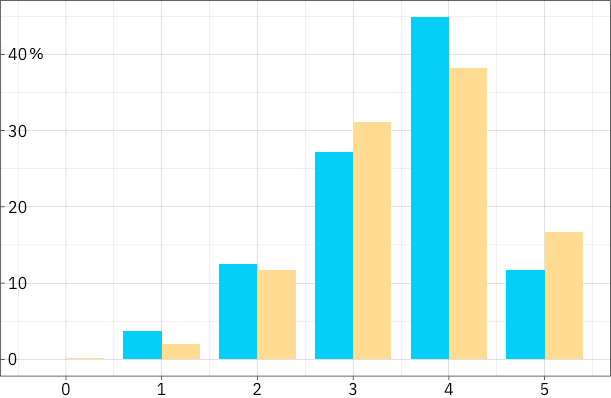
\includegraphics{imgs/edit_distance_reais.png}
  \caption{\textit{Edit-distances} das organizações coletadas (em azul) \textit{vs} uma organização ``aleatória'' (em amarelo).}
  \label{edit_dist_1}
\end{marginfigure}

Aqui, não pudemos intuir se nos dados estávamos vendo que nossa tipografia modulada pela fala era ineficaz ou se estávamos sofrendo com o mau desenho do experimento. Talvez, apostamos, seja mais o segundo caso: o modo como configuramos o \textit{card sort} pode ter conduzido a altas taxas de erro. Como \textit{todos} os cartões deveriam necessariamente ser atribuídos a uma emoção, estão embaralhados em nossos resultados coletados tanto cartões em que o participante tinha algum grau de certeza sobre a emoção quanto aqueles em que houve um ``chute.''\sidenote[][-1\baselineskip]{E, para piorar, no \textit{card sort} um cartão errado implicará necessariamente em um segundo cartão também errado.} Temos motivos para crer que esses chutes foram comuns, pois, tanto nas entrevistas quanto espontaneamente durante a atividade, muitos participantes nos relataram que a atividade era muito difícil.

A essa dificuldade da atividade em si soma-se o fato de que misturamos no experimento, e sem nenhuma forma de controle que isolassem seus efeitos, variações de três \textit{features} prosódicas com três eixos tipográficos associados a seis emoções. Dado esse cenário, não é de se espantar que com os dados coletados nos foi muito difícil responder quão bem (ou mal) nosso modelo prosódico-tipográfico representava a voz da atriz em cada uma das emoções presentes. 


\begin{marginfigure}
  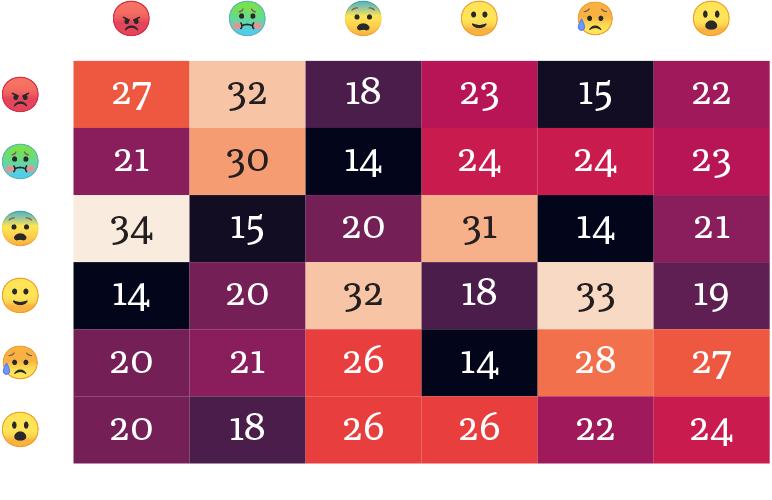
\includegraphics{imgs/confusion-emoji2.png}
  \caption{Matriz de confusão do experimento de \textit{card sort}. Emoção da atriz nas linhas, classificação dos participantes nas colunas.}
  \label{matriz_confusao}
\end{marginfigure}

Na tentativa de encontrar explicações alternativas para o baixo ganho no \textit{edit-distance}, nos perguntarmos se certos aspectos do modelo prosódico-tipográfico não estariam fazendo os participantes trocarem uma emoção por outra. Esta hipótese nos ocorreu na análise da matriz de confusão da Figura~\ref{matriz_confusao}, que parece indicar uma possível troca feita pelos participantes especificamente entre os cartões representando medo e alegria (terceira e quarta linhas e colunas). Teria o modelo invertido o sentido de alguma das features ou eixos tipográficos em relação ao que seria intuitivo? Para testar a hipótese, calculamos novamente a \textit{edit-distance}, desta vez considerando que os cartões com medo seriam de alegria e vice-versa. Como mostra a Figura~\ref{edit_dist_2}, a performance melhora (8\% de ganho em relação à distribuição aleatória). Mas o efeito continua pequeno.

\begin{marginfigure}[0.5\baselineskip]
  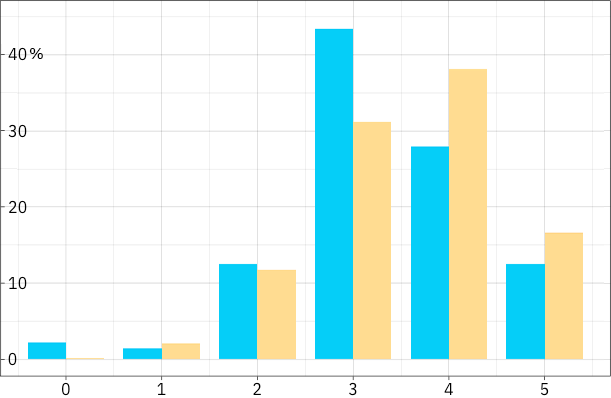
\includegraphics{imgs/edit_distance_troca.png}
  \caption{\textit{Edit-distances} das organizações coletadas, mas com troca alegria--medo (em azul) \textit{vs} uma organização ``aleatória'' (em amarelo).}
  \label{edit_dist_2}
\end{marginfigure}

O que nos disseram as entrevistas? Além do muito frequente comentário de que a avaliação era muito difícil, emergiram alguns padrões em como os participantes interpretaram as modulações tipográficas. De longe o atributo mais citado, aumento no \textit{peso} foi quase unanimemente associado a maior volume na voz, ainda que foram poucos os que perceberam que pesos leves estavam relacionados a volumes baixos na voz.

Em relação aos outros dois eixos houve grande difusão de comentários. Sobre a \textit{inclinação}, houve quem a interpretasse como velocidade, fraqueza, tristeza, ou mesmo alguns que notaram as modulações nesse eixo mas que não souberam decodificá-las. \textit{Largura} foi citada por apenas um participante, que intuiu corretamente que seu aumento e baixa estavam relacionados a oscilações de duração na pronúncia das sílabas.

Comentando sobre estratégias usadas para classificar cada cartão, emergiram dois principais grupos: no primeiro, mais frequente, o participante olhava para o cartão e buscava ``soá-lo'' mentalmente\sidenote{Ou, mais raramente, em voz baixa, como notamos em alguns casos.}, tentando interpretar em sons as modulações visuais nas letras. O segundo grupo ia no sentido oposto: tentava fazer soar a frase como que sob o efeito de cada uma das seis emoções para só então buscar nos cartões aquele cuja tipografia se aproximasse do som.

Como muitos participantes sequer perceberam as modulações de \textit{largura} e que houve grande divergência em como foram interpretadas as modulações de \textit{inclinação}, podemos supor que ambas as estratégias relatadas sofrem de um mesmo problema: se apenas os momentos mais gritados foram bem capturados, grande parte da expressividade na voz da atriz se perdeu e, não só isso, essa perda compromete de maneira desigual cada uma das emoções.\sidenote[][-2\baselineskip]{\citet{deMoraes2016} mostram como variações nas \textit{features} de $f_0$ e duração são sensíveis à expressão de diferentes emoções na voz.}

\subsection{O segundo experimento}

Os resultados do segundo experimento, sintetizados na tabela~\ref{tab:type_perf}, são mais esclarecedores. Ao cruzar como interagem as dimensões emoção na voz, \textit{feature} prosódica e eixo tipográfico, é possível perceber que as preferências dos participantes não seguem um padrão único, variando de acordo com as diferentes possíveis combinações dessas dimensões. Pode-se vislumbrar assim que uma representação bem sucedida de qualidades expressivas da prosódia teria que ponderar os atributos dessa mesma prosódia para só então determinar quais eixos tipográficos modular.


\begin{table}
    \small
    \caption{Preferência dos participantes por cada modulação tipográfica quando usada com cada uma das emoções (considerando a média entre as duas frases testadas). \newline A preferência de 83\% para \textit{peso} quando usado para representar \textsc{rms} na frase com raiva, por exemplo, indica que ela foi escolhida em 83\% das vezes em que foi colocada contra os outros três eixos. \newline Células em verde indicam que uma dada combinação de eixo tipográfico e \textit{feature} prosódica obteve a maior preferência dentre todas as possibilidades testadas. Células em cinza indica maior preferência apenas para aquela determinada \textit{feature}. \newline Não elegemos uma preferência para tristeza pois nela a distribuição das preferências não foi estatisticamente significante.}
    \label{tab:type_perf}
    \begin{center}
    \resizebox{.93\textwidth}{!}{%
    \begin{tabular}{lcccc}
        \toprule
        \multicolumn{5}{c}{ \textbf{\textsc{rms} enquanto \textit{feature} representada.} }     \\
        \midrule
        emoção na voz & weight & width & slant & baseline shift  \\
        \midrule
        raiva & \cellcolor[HTML]{dddddd}83\% & 34\% & 43\% & 39\% \\
        alegria & 34\% & 54\% & 47\% & \cellcolor[HTML]{dddddd}64\% \\
        neutra & 47\% & 52\% & \cellcolor[HTML]{9ef7cd}76\% & 25\% \\
        tristeza & 45\% & 52\% & 46\% & 58\% \\
        surpresa & \cellcolor[HTML]{9ef7cd}72\% & 38\% & 49\% & 43\% \\
        \midrule
        \multicolumn{5}{c}{ \textbf{\textit{f\textsubscript{0}} enquanto \textit{feature} representada.} }      \\
        \midrule
        emoção na voz & weight & width & slant & baseline shift  \\
        \midrule
        raiva & \cellcolor[HTML]{9ef7cd}87\% & 46\% & 45\% & 26\% \\
        alegria & 28\% & 66\% & 40\% & \cellcolor[HTML]{9ef7cd}69\% \\
        neutra & 47\% & 55\% & \cellcolor[HTML]{dddddd}63\% & 35\% \\
        tristeza & 21\% & 57\% & 39\% & \cellcolor[HTML]{9ef7cd}79\% \\
        surpresa & \cellcolor[HTML]{dddddd}71\% & 43\% & 41\% & 44\% \\
        \bottomrule
    \end{tabular}}
    \end{center}
\end{table}

Essa constatação, se verdadeira, carrega uma explicação possível para pelo menos parte do insucesso na abordagem testada no primeiro experimento: ao combinar sempre da mesma maneira as três \textit{features} prosódicas com os mesmos três eixos tipográficos, tínhamos uma tipografia que coincidia com as expectativas dos participantes apenas em parte dos cartões.

Por exemplo: se, como nos mostra a tabela~\ref{tab:type_perf}, as pessoas não acham que o eixo \textit{peso} produz boas representações do \textsc{rms} em uma voz feliz, o fato de que assim o usávamos também nos cartões em que a atriz simulou felicidade pode tê-los aproximado da raiva ou da surpresa, emoções onde o \textit{peso} parece mais apropriado.

\begin{marginfigure}[15\baselineskip]
  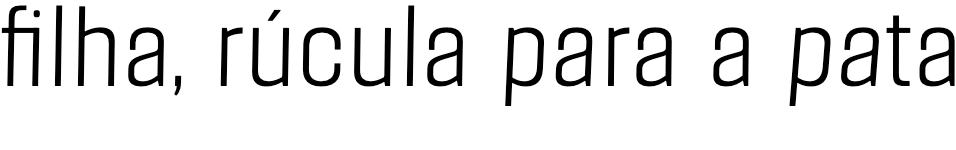
\includegraphics{imgs/slight-slant.png}
  \caption{\textit{Inclinação} como representação de \textsc{rms} na versão neutra da frase.}
  \label{slight_slant}
\end{marginfigure}

Outra conclusão interessante é que tanto \textit{largura horizontal} quando \textit{inclinação}, pouco citados nas entrevistas do primeiro experimento, tem em geral uma performance mediana, com a preferência geral tendendo à inclinação apenas quando esta é associada a uma emoção que é diferente de todas as outras: a voz neutra. De fato, como pode-se notar na figura~\ref{slight_slant}, eleita a representação mais fiel da voz neutra, as modulações tipográficas aqui são praticamente imperceptíveis. Mas esse resultado não estranha: talvez estas tenham sido as escolhas dos participantes justamente porque, em vozes que buscam ser inexpressivas, as melhores representações seriam aquelas nas quais quase não haja modulação tipográfica. Se for mesmo esse o caso, pode-se supor que uma abordagem que pondere os atributos prosódicos para só então determinar quais eixos tipográficos modular deve considerar também a possibilidade de, para determinadas vozes, \textit{não modular eixo algum}.

Se quando fizemos o primeiro e segundo experimentos ainda não conhecíamos alternativas mais robustas que o \textsc{rms} para medir intensidade, na análise dos dados do segundo experimento nos pareceu oportuno nos aproveitarmos da medida obtida pela distância entre a Frequência fundamental ($f_0$) e a Centroide espectral ($C-f_0$) -- \textit{feature} com a qual havíamos acabado de ter contato que, como \textsc{rms}, está relacionada à intensidade, mas que ao contrário desta captura o esforço vocal do falante com maior independência de particularidades do ambiente de gravação. Apesar de que a \textit{feature} não foi utilizada para modular a tipografia, os participantes tiveram acesso aos áudios originais, de onde por suposto conseguiram deduzir o esforço vocal da atriz o que, supomos, entrou em consideração em suas escolhas.

\begin{marginfigure}[-2\baselineskip]
  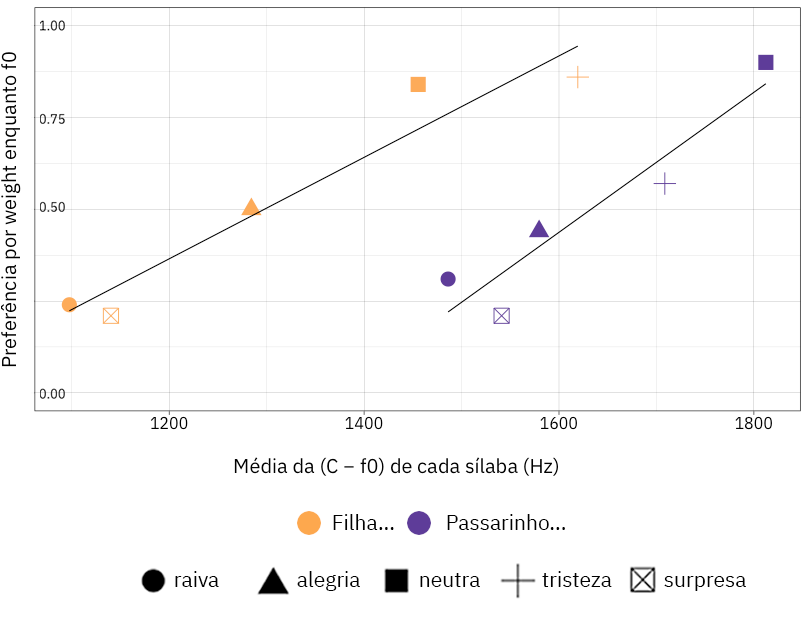
\includegraphics{imgs/weight--f0.png}
  \caption{Relação entre performance de \textit{weight} e $C-f_0$}
  \label{weight_as_f0}
\end{marginfigure}

Na figura~\ref{weight_as_f0}, mostramos como a performance do eixo \textit{weight}, quando usado para representar a $f_0$, está relacionado ao valor $C-f_0$ médio de cada frase. Para a frase ``Filha'', encontramos uma equação de regressão significante\sidenote[][2\baselineskip]{``Filha'': (F(1,3)=39.27, p<0.05), \textsc{rse}=0.09; ``Passarinho'': (F(1,3)=24.07, p<0.05), \textsc{rse}=0.10} com um $R^2$ de 0,93 e fórmula de performance de $(C-f_0) * 10^{-3} - 1,29$. Para a frase ``Passarinho'', também encontramos uma equação de regressão significante com um $R^2$ de 0,89 e fórmula de performance de $(C-f_0) * 10^{-3} - 2,61$.

Já na figura~\ref{baseline_shift_as_f0}, tomamos a performance do eixo \textit{baseline shift} representando $f_0$ e a relacionamos às mudanças de $C - f_0$ nas duas frases. As retas aqui se invertem, e as preferências dos participantes estão inversamente correlacionadas aos valores de $C-f_0$, ainda que neste caso as equações de regressão não tenham sido significantes\footnote{``Filha'': (F(1,3)=1.36, p=0.33), \textsc{rse}=0.23; ``Passarinho'': (F(1,3)=5.26, p=0.11), \textsc{rse}=0.16} -- são, portanto, mostradas como linhas tracejadas.

\begin{marginfigure}[2\baselineskip]
  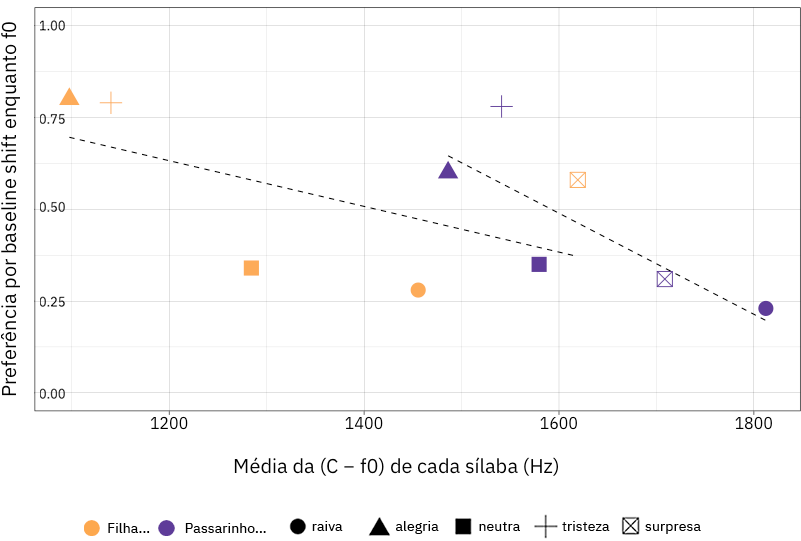
\includegraphics{imgs/baseline_shift--f0.png}
  \caption{Relação entre performance de \textit{baseline shift} e $C-f_0$}
  \label{baseline_shift_as_f0}
\end{marginfigure}

Sintetizando os dois achados, vemos que conforme aumenta o esforço vocal no áudio aumenta também a preferência pelo uso do eixo \textit{weight}. Em frases ditas com menor intensidade os participantes preferem, ainda que de maneira mais difusa, o uso do \textit{baseline shift}.

Uma última discussão se dá com os comentários deixados pelos participantes. Muitos desses textos discorrem sobre como foram interpretadas as modulações tipográficas. Notamos que cada eixo foi associado a diversas qualidades -- agressividade e firmeza para o \textit{peso}; uma voz melódica, quase cantada, ou divertida, ou ainda bêbada para o \textit{deslocamento vertical}; uma voz tímida para a~\textit{largura horizontal;} etc. 

Surge que, nesse compêndio de qualidades, mesmo que as respostas tenham vindo difusas, cada uma trazendo adjetivos diferentes entre si, de um modo geral os participantes parecem não estar descrevendo os atributos \textit{acústicos} da prosódia que os eixos tipográficos representavam e tampouco as seis emoções que a atriz buscou representar. Antes, as descrições falam de vozes \textit{modificadas}, como se os participantes não tenham deduzido nem nosso modelo prosódico-tipográfico nem, como esperávamos no primeiro experimento, as emoções que a atriz buscou representar, mas sim uma interpretação própria que assimila emoção \textit{e}~acústica.

Esse resultado condiz com o que discutem Boehner et al. quando apontam que ``a comunicação de afetos em um modelo interacional (...) é mais do que a mera transmissão, (...) requerindo das partes uma interpretação ativa.'' \sidenote[][-1\baselineskip]{\begin{otherlanguage}{english}\textit{[C]ommunication of affect in an interactional model (...) is more than transmission, [and] requires active interpretation.}\end{otherlanguage}  \citep{boehner2005affect}} A partir desta perspectiva, pode-se enquadrar melhor o propósito de um sistema construído a partir de nosso modelo prosódico-tipográfico: não querê-lo como uma maneira de informar ao leitor que em dada frase a voz representava esta ou aquela emoção, categórica e de contornos bem definidos, mas sim usar a tipografia como maneira de ressaltar aspectos expressivos na voz, ambíguos como a própria voz e, como ela, abertos a~múltiplas interpretações. Ainda segundo Boehner et al., a ``medida de sucesso de tais sistemas [como o nosso] está então não no fato de que deduzem ou não a emoção `correta', mas em se provocam o reconhecimento e reflexão sobre emoções em seus usuários.'' \sidenote[][-4\baselineskip]{\begin{otherlanguage}{english}\textit{Measures of success for such systems are therefore not whether the systems themselves deduce the `right' emotion but whether the systems encourage awareness of and reflection on emotions in users.}\end{otherlanguage} \citep{boehner2005affect}}




\renewcommand{\refname}{Bibliografia}
\makeatletter
\renewcommand{\bibsection}{%
   \section{\refname%
            \@mkboth{\MakeUppercase{\refname}}{\MakeUppercase{\refname}}%
   }
}
\makeatother


\bibliography{refs}
\bibliographystyle{apalike}
%\bibliographystyle{plainnat}
%\bibliographystyle{agsm}


\end{document}